\documentclass[11pt]{article}
\usepackage[OT4]{fontenc}
\newtheorem{define}{Definition}
\usepackage{graphicx}
\usepackage{subcaption}
\usepackage{hyperref}
\usepackage{booktabs}
\usepackage{amsmath}
\usepackage{stackengine}
\usepackage{amsfonts}
\usepackage{amssymb}
\oddsidemargin=0.15in
\evensidemargin=0.15in
\topmargin=-.5in
\textheight=9in
\textwidth=6.25in

\begin{document}
	
%--------------
%% preamble.tex
%% this should be included with a command like
%% %--------------
%% preamble.tex
%% this should be included with a command like
%% %--------------
%% preamble.tex
%% this should be included with a command like
%% \input{preamble.tex}
%% Template based on Aleksander Madry's and Dan Spielman's template

\hbadness=10000
\vbadness=10000

\setlength{\oddsidemargin}{.25in}
\setlength{\evensidemargin}{.25in}
\setlength{\textwidth}{6in}
\setlength{\topmargin}{-0.4in}
\setlength{\textheight}{8.5in}

\newcommand{\handout}[5]{
	\noindent
	\begin{center}
		\framebox{
			\vbox{
				\hbox to 5.78in { {\bf #1}
					\hfill #2 }
				\vspace{4mm}
				\hbox to 5.78in { {\Large \hfill #5  \hfill} }
				\vspace{2mm}
				\hbox to 5.78in { {\it #3 \hfill #4} }
			}
		}
	\end{center}
	\vspace*{4mm}
}

\newcommand{\header}[2]{\handout{NUS CS4243: Computer Vision and Pattern Recognition}{\today}{Lecturer: Angela Yao;}{Students: #1}{#2}}


\newtheorem{theorem}{Theorem}
\newtheorem{corollary}[theorem]{Corollary}
\newtheorem{lemma}[theorem]{Lemma}
\newtheorem{observation}[theorem]{Observation}
\newtheorem{proposition}[theorem]{Proposition}
\newtheorem{definition}[theorem]{Definition}
\newtheorem{claim}[theorem]{Claim}
\newtheorem{fact}[theorem]{Fact}
\newtheorem{assumption}[theorem]{Assumption}

\newcommand{\qed}{\rule{7pt}{7pt}}
\newcommand{\dis}{\mathop{\mbox{\rm d}}\nolimits}
\newcommand{\per}{\mathop{\mbox{\rm per}}\nolimits}
\newcommand{\area}{\mathop{\mbox{\rm area}}\nolimits}
\newcommand{\cw}{\mathop{\rm cw}\nolimits}
\newcommand{\ccw}{\mathop{\rm ccw}\nolimits}
\newcommand{\DIST}{\mathop{\mbox{\rm DIST}}\nolimits}
\newcommand{\OP}{\mathop{\mbox{\it OP}}\nolimits}
\newcommand{\OPprime}{\mathop{\mbox{\it OP}^{\,\prime}}\nolimits}
\newcommand{\ihat}{\hat{\imath}}
\newcommand{\jhat}{\hat{\jmath}}
\newcommand{\abs}[1]{\mathify{\left| #1 \right|}}

\newenvironment{proof}{\noindent{\bf Proof}\hspace*{1em}}{\qed\bigskip}
\newenvironment{proof-sketch}{\noindent{\bf Sketch of Proof}\hspace*{1em}}{\qed\bigskip}
\newenvironment{proof-idea}{\noindent{\bf Proof Idea}\hspace*{1em}}{\qed\bigskip}
\newenvironment{proof-of-lemma}[1]{\noindent{\bf Proof of Lemma #1}\hspace*{1em}}{\qed\bigskip}
\newenvironment{proof-attempt}{\noindent{\bf Proof Attempt}\hspace*{1em}}{\qed\bigskip}
\newenvironment{proofof}[1]{\noindent{\bf Proof}
of #1:\hspace*{1em}}{\qed\bigskip}
\newenvironment{remark}{\noindent{\bf Remark}\hspace*{1em}}{\bigskip}

% \makeatletter
% \@addtoreset{figure}{section}
% \@addtoreset{table}{section}
% \@addtoreset{equation}{section}
% \makeatother

\newcommand{\FOR}{{\bf for}}
\newcommand{\TO}{{\bf to}}
\newcommand{\DO}{{\bf do}}
\newcommand{\WHILE}{{\bf while}}
\newcommand{\AND}{{\bf and}}
\newcommand{\IF}{{\bf if}}
\newcommand{\THEN}{{\bf then}}
\newcommand{\ELSE}{{\bf else}}

% \renewcommand{\thefigure}{\thesection.\arabic{figure}}
% \renewcommand{\thetable}{\thesection.\arabic{table}}
% \renewcommand{\theequation}{\thesection.\arabic{equation}}

\makeatletter
\def\fnum@figure{{\bf Figure \thefigure}}
\def\fnum@table{{\bf Table \thetable}}
\long\def\@mycaption#1[#2]#3{\addcontentsline{\csname
  ext@#1\endcsname}{#1}{\protect\numberline{\csname 
  the#1\endcsname}{\ignorespaces #2}}\par
  \begingroup
    \@parboxrestore
    \small
    \@makecaption{\csname fnum@#1\endcsname}{\ignorespaces #3}\par
  \endgroup}
\def\mycaption{\refstepcounter\@captype \@dblarg{\@mycaption\@captype}}
\makeatother

\newcommand{\figcaption}[1]{\mycaption[]{#1}}
\newcommand{\tabcaption}[1]{\mycaption[]{#1}}
\newcommand{\head}[1]{\chapter[Lecture \##1]{}}
\newcommand{\mathify}[1]{\ifmmode{#1}\else\mbox{$#1$}\fi}
%\renewcommand{\Pr}[1]{\mathify{\mbox{Pr}\left[#1\right]}}
%\newcommand{\Exp}[1]{\mathify{\mbox{Exp}\left[#1\right]}}
\newcommand{\bigO}O
\newcommand{\set}[1]{\mathify{\left\{ #1 \right\}}}
\def\half{\frac{1}{2}}

\newcommand{\fig}[4]{
        \begin{figure}
        \setlength{\epsfysize}{#2}
        \vspace{3mm}
        \centerline{\epsfbox{#4}}
        \caption{#3} \label{#1}
        \end{figure}
        }

\newcommand{\ord}{{\rm ord}}

\providecommand{\norm}[1]{\lVert #1 \rVert}
\newcommand{\embed}{{\rm Embed}}
\newcommand{\qembed}{\mbox{$q$-Embed}}
\newcommand{\calh}{{\cal H}}
\newcommand{\lp}{{\rm LP}}

%% Template based on Aleksander Madry's and Dan Spielman's template

\hbadness=10000
\vbadness=10000

\setlength{\oddsidemargin}{.25in}
\setlength{\evensidemargin}{.25in}
\setlength{\textwidth}{6in}
\setlength{\topmargin}{-0.4in}
\setlength{\textheight}{8.5in}

\newcommand{\handout}[5]{
	\noindent
	\begin{center}
		\framebox{
			\vbox{
				\hbox to 5.78in { {\bf #1}
					\hfill #2 }
				\vspace{4mm}
				\hbox to 5.78in { {\Large \hfill #5  \hfill} }
				\vspace{2mm}
				\hbox to 5.78in { {\it #3 \hfill #4} }
			}
		}
	\end{center}
	\vspace*{4mm}
}

\newcommand{\header}[2]{\handout{NUS CS4243: Computer Vision and Pattern Recognition}{\today}{Lecturer: Angela Yao;}{Students: #1}{#2}}


\newtheorem{theorem}{Theorem}
\newtheorem{corollary}[theorem]{Corollary}
\newtheorem{lemma}[theorem]{Lemma}
\newtheorem{observation}[theorem]{Observation}
\newtheorem{proposition}[theorem]{Proposition}
\newtheorem{definition}[theorem]{Definition}
\newtheorem{claim}[theorem]{Claim}
\newtheorem{fact}[theorem]{Fact}
\newtheorem{assumption}[theorem]{Assumption}

\newcommand{\qed}{\rule{7pt}{7pt}}
\newcommand{\dis}{\mathop{\mbox{\rm d}}\nolimits}
\newcommand{\per}{\mathop{\mbox{\rm per}}\nolimits}
\newcommand{\area}{\mathop{\mbox{\rm area}}\nolimits}
\newcommand{\cw}{\mathop{\rm cw}\nolimits}
\newcommand{\ccw}{\mathop{\rm ccw}\nolimits}
\newcommand{\DIST}{\mathop{\mbox{\rm DIST}}\nolimits}
\newcommand{\OP}{\mathop{\mbox{\it OP}}\nolimits}
\newcommand{\OPprime}{\mathop{\mbox{\it OP}^{\,\prime}}\nolimits}
\newcommand{\ihat}{\hat{\imath}}
\newcommand{\jhat}{\hat{\jmath}}
\newcommand{\abs}[1]{\mathify{\left| #1 \right|}}

\newenvironment{proof}{\noindent{\bf Proof}\hspace*{1em}}{\qed\bigskip}
\newenvironment{proof-sketch}{\noindent{\bf Sketch of Proof}\hspace*{1em}}{\qed\bigskip}
\newenvironment{proof-idea}{\noindent{\bf Proof Idea}\hspace*{1em}}{\qed\bigskip}
\newenvironment{proof-of-lemma}[1]{\noindent{\bf Proof of Lemma #1}\hspace*{1em}}{\qed\bigskip}
\newenvironment{proof-attempt}{\noindent{\bf Proof Attempt}\hspace*{1em}}{\qed\bigskip}
\newenvironment{proofof}[1]{\noindent{\bf Proof}
of #1:\hspace*{1em}}{\qed\bigskip}
\newenvironment{remark}{\noindent{\bf Remark}\hspace*{1em}}{\bigskip}

% \makeatletter
% \@addtoreset{figure}{section}
% \@addtoreset{table}{section}
% \@addtoreset{equation}{section}
% \makeatother

\newcommand{\FOR}{{\bf for}}
\newcommand{\TO}{{\bf to}}
\newcommand{\DO}{{\bf do}}
\newcommand{\WHILE}{{\bf while}}
\newcommand{\AND}{{\bf and}}
\newcommand{\IF}{{\bf if}}
\newcommand{\THEN}{{\bf then}}
\newcommand{\ELSE}{{\bf else}}

% \renewcommand{\thefigure}{\thesection.\arabic{figure}}
% \renewcommand{\thetable}{\thesection.\arabic{table}}
% \renewcommand{\theequation}{\thesection.\arabic{equation}}

\makeatletter
\def\fnum@figure{{\bf Figure \thefigure}}
\def\fnum@table{{\bf Table \thetable}}
\long\def\@mycaption#1[#2]#3{\addcontentsline{\csname
  ext@#1\endcsname}{#1}{\protect\numberline{\csname 
  the#1\endcsname}{\ignorespaces #2}}\par
  \begingroup
    \@parboxrestore
    \small
    \@makecaption{\csname fnum@#1\endcsname}{\ignorespaces #3}\par
  \endgroup}
\def\mycaption{\refstepcounter\@captype \@dblarg{\@mycaption\@captype}}
\makeatother

\newcommand{\figcaption}[1]{\mycaption[]{#1}}
\newcommand{\tabcaption}[1]{\mycaption[]{#1}}
\newcommand{\head}[1]{\chapter[Lecture \##1]{}}
\newcommand{\mathify}[1]{\ifmmode{#1}\else\mbox{$#1$}\fi}
%\renewcommand{\Pr}[1]{\mathify{\mbox{Pr}\left[#1\right]}}
%\newcommand{\Exp}[1]{\mathify{\mbox{Exp}\left[#1\right]}}
\newcommand{\bigO}O
\newcommand{\set}[1]{\mathify{\left\{ #1 \right\}}}
\def\half{\frac{1}{2}}

\newcommand{\fig}[4]{
        \begin{figure}
        \setlength{\epsfysize}{#2}
        \vspace{3mm}
        \centerline{\epsfbox{#4}}
        \caption{#3} \label{#1}
        \end{figure}
        }

\newcommand{\ord}{{\rm ord}}

\providecommand{\norm}[1]{\lVert #1 \rVert}
\newcommand{\embed}{{\rm Embed}}
\newcommand{\qembed}{\mbox{$q$-Embed}}
\newcommand{\calh}{{\cal H}}
\newcommand{\lp}{{\rm LP}}

%% Template based on Aleksander Madry's and Dan Spielman's template

\hbadness=10000
\vbadness=10000

\setlength{\oddsidemargin}{.25in}
\setlength{\evensidemargin}{.25in}
\setlength{\textwidth}{6in}
\setlength{\topmargin}{-0.4in}
\setlength{\textheight}{8.5in}

\newcommand{\handout}[5]{
	\noindent
	\begin{center}
		\framebox{
			\vbox{
				\hbox to 5.78in { {\bf #1}
					\hfill #2 }
				\vspace{4mm}
				\hbox to 5.78in { {\Large \hfill #5  \hfill} }
				\vspace{2mm}
				\hbox to 5.78in { {\it #3 \hfill #4} }
			}
		}
	\end{center}
	\vspace*{4mm}
}

\newcommand{\header}[2]{\handout{NUS CS4243: Computer Vision and Pattern Recognition}{\today}{Lecturer: Angela Yao;}{Students: #1}{#2}}


\newtheorem{theorem}{Theorem}
\newtheorem{corollary}[theorem]{Corollary}
\newtheorem{lemma}[theorem]{Lemma}
\newtheorem{observation}[theorem]{Observation}
\newtheorem{proposition}[theorem]{Proposition}
\newtheorem{definition}[theorem]{Definition}
\newtheorem{claim}[theorem]{Claim}
\newtheorem{fact}[theorem]{Fact}
\newtheorem{assumption}[theorem]{Assumption}

\newcommand{\qed}{\rule{7pt}{7pt}}
\newcommand{\dis}{\mathop{\mbox{\rm d}}\nolimits}
\newcommand{\per}{\mathop{\mbox{\rm per}}\nolimits}
\newcommand{\area}{\mathop{\mbox{\rm area}}\nolimits}
\newcommand{\cw}{\mathop{\rm cw}\nolimits}
\newcommand{\ccw}{\mathop{\rm ccw}\nolimits}
\newcommand{\DIST}{\mathop{\mbox{\rm DIST}}\nolimits}
\newcommand{\OP}{\mathop{\mbox{\it OP}}\nolimits}
\newcommand{\OPprime}{\mathop{\mbox{\it OP}^{\,\prime}}\nolimits}
\newcommand{\ihat}{\hat{\imath}}
\newcommand{\jhat}{\hat{\jmath}}
\newcommand{\abs}[1]{\mathify{\left| #1 \right|}}

\newenvironment{proof}{\noindent{\bf Proof}\hspace*{1em}}{\qed\bigskip}
\newenvironment{proof-sketch}{\noindent{\bf Sketch of Proof}\hspace*{1em}}{\qed\bigskip}
\newenvironment{proof-idea}{\noindent{\bf Proof Idea}\hspace*{1em}}{\qed\bigskip}
\newenvironment{proof-of-lemma}[1]{\noindent{\bf Proof of Lemma #1}\hspace*{1em}}{\qed\bigskip}
\newenvironment{proof-attempt}{\noindent{\bf Proof Attempt}\hspace*{1em}}{\qed\bigskip}
\newenvironment{proofof}[1]{\noindent{\bf Proof}
of #1:\hspace*{1em}}{\qed\bigskip}
\newenvironment{remark}{\noindent{\bf Remark}\hspace*{1em}}{\bigskip}

% \makeatletter
% \@addtoreset{figure}{section}
% \@addtoreset{table}{section}
% \@addtoreset{equation}{section}
% \makeatother

\newcommand{\FOR}{{\bf for}}
\newcommand{\TO}{{\bf to}}
\newcommand{\DO}{{\bf do}}
\newcommand{\WHILE}{{\bf while}}
\newcommand{\AND}{{\bf and}}
\newcommand{\IF}{{\bf if}}
\newcommand{\THEN}{{\bf then}}
\newcommand{\ELSE}{{\bf else}}

% \renewcommand{\thefigure}{\thesection.\arabic{figure}}
% \renewcommand{\thetable}{\thesection.\arabic{table}}
% \renewcommand{\theequation}{\thesection.\arabic{equation}}

\makeatletter
\def\fnum@figure{{\bf Figure \thefigure}}
\def\fnum@table{{\bf Table \thetable}}
\long\def\@mycaption#1[#2]#3{\addcontentsline{\csname
  ext@#1\endcsname}{#1}{\protect\numberline{\csname 
  the#1\endcsname}{\ignorespaces #2}}\par
  \begingroup
    \@parboxrestore
    \small
    \@makecaption{\csname fnum@#1\endcsname}{\ignorespaces #3}\par
  \endgroup}
\def\mycaption{\refstepcounter\@captype \@dblarg{\@mycaption\@captype}}
\makeatother

\newcommand{\figcaption}[1]{\mycaption[]{#1}}
\newcommand{\tabcaption}[1]{\mycaption[]{#1}}
\newcommand{\head}[1]{\chapter[Lecture \##1]{}}
\newcommand{\mathify}[1]{\ifmmode{#1}\else\mbox{$#1$}\fi}
%\renewcommand{\Pr}[1]{\mathify{\mbox{Pr}\left[#1\right]}}
%\newcommand{\Exp}[1]{\mathify{\mbox{Exp}\left[#1\right]}}
\newcommand{\bigO}O
\newcommand{\set}[1]{\mathify{\left\{ #1 \right\}}}
\def\half{\frac{1}{2}}

\newcommand{\fig}[4]{
        \begin{figure}
        \setlength{\epsfysize}{#2}
        \vspace{3mm}
        \centerline{\epsfbox{#4}}
        \caption{#3} \label{#1}
        \end{figure}
        }

\newcommand{\ord}{{\rm ord}}

\providecommand{\norm}[1]{\lVert #1 \rVert}
\newcommand{\embed}{{\rm Embed}}
\newcommand{\qembed}{\mbox{$q$-Embed}}
\newcommand{\calh}{{\cal H}}
\newcommand{\lp}{{\rm LP}}

\header{Maximilian Fruehauf, David Drews, Choo Wen Xin}{Where's Waldo Detector using Computer Vision}

\begin{abstract}
This report describes our group's implementation of a computer vision algorithm to detect the three
characters Waldo, Wenda, Wizard in a series of high-resolution scans taken from the "Where's Waldo"
books. Due to the complex nature of the illustrations, the variation of the characters' appearances
and the constraint to use non-deep learning techniques only, detecting the characters accurately
proved to be a challenge. We combined a histogram over gradients (HoG) with a histogram over values
(HoV) feature descriptor to train a SVM find the characters in the images. While being able to
detect a decent amount of Waldos and Wendas, our SVM only detects a few Wizards which correlates to
the number of training samples available for each class.
\end{abstract}

%%%% body goes in here %%%%
\section{Introduction}

"Where's Waldo" is a series of books containing detailed, high-resolution illustrations. The
illustrations are characterised by showing a large number of people pursuing various activities in an
often themed environment. The reader must find the characters who may or may not appear on any given
page. For this project, we are given a set of scanned images from the books and are tasked to design a
computer vision algorithm that can detect the three characters from the book: Waldo, Wenda, and the
Wizard. We are provided with a set of training images with annotations of the bounding box locations of
Waldo, Wenda and Wizard in each image.\\

Throughout the course of the project, we attempted several different methods with varying degrees
of success due to the difficult nature of the task. While there are several existing computer vision
algorithms for object detection in general and face detection specifically, such as the "You Only Look
Once" object detection~\cite{redmon2016yolo}, we were not allowed to use deep learning based approaches
in this project. As the characters are illustrated, face detection classifiers that were pre-trained
with human faces weren't performing well in our problem domain. Lastly, the characters' appearance and size
varies a lot across images. For example, sometimes only a smaller part of the character such as part
of the face is visible and the rest is covered contents within the image. These boundary conditions
make finding and identifying the characters very challenging.\\

Across all approaches, we only worked with the data that was handed to us as part of the assignment.
Although our code alters the given data wherever needed, we did neither add any entirely new data from
sources like the internet nor did we manually improve the existing data as could be achieved by adding
or improving annotations.\\

We proposed focusing on the following methods which we will explain in the next section:

\begin{itemize}
    \item histogram over gradients (HoG) feature descriptor
    \item histogram over values (HoV) feature descriptor
    \item training a linear support vector machine (SVM) to create a multiclass-classifier
\end{itemize}

\section{Proposed Solution}
Our proposed solution has two phases: pre-processing and detection.\\

In the pre-processing phase, we will take all the provided high-resolution training images and crop out the three characters using
the given input bounding box annotations. Negative samples will be obtained by arbitiarily sampling
regions from the images that do not overlap with the given character bounding boxes. We will scale
all these images to a fixed size for simplification. We will then run k-means preprocessing on these
images to map the colored sample images to grayscale values. The details will be further discussed in
\autoref{subsec:data-prep}.\\

Our detection phase first involves histogramming two types of feature descriptors: gradients (HoG) and
values (HoV). HoG will be used to histogram horizontal and vertical gradients in the image, which could
be quite helpful in identifying features like the horizontal stripes in Waldo and Wenda's shirts. HoV is
to histogram values from a SIFT detector. We will use our training samples to train support vector
machines (SVM) as a classifier to determine whether a window is either \(Waldo, Wenda, Wizard or Negative\).
The classifier will predict a probability \(p\) that a window belongs to a certain class, and a ratio
\(p_{ratio}\) to indicate the classifier's confidence in ratio to the other classes.
In the next step, we will perform non-maximum supression to rermove overlapping windows by choosing the
one with the highest probability in each group. Finally, the resulting boxes with the class label will
be drawn on the image with the value of its probability and ratio as illustrated in
\autoref{fig:waldo-winter}. The details will be further discussed in \autoref{subsec:implementation}.

\begin{figure}[h]
    \centering
    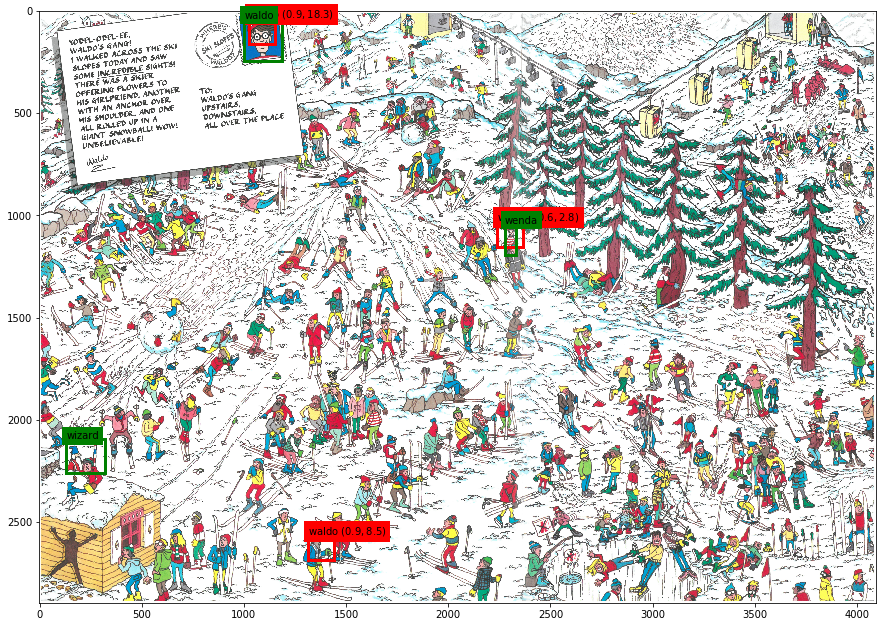
\includegraphics[width=0.8\linewidth]{figures/waldo_winter} 
    \caption{Image showing detections with \( (name, p, p_{ratio}) \) in red, ground truth in green.}
    \label{fig:waldo-winter}
\end{figure}

\section{Experiments}
\subsection{Data Preparation and Configuration}\label{subsec:data-prep}

The images in the dataset come as annotated bounding boxes of varying aspect ratios and sizes in pixels.
Also the size of the respective images changes as well. Therefore we simplified the detection process by
generating \( (128 \times 128) \) px training images from the provided bounding boxes. 
Doing so resulted in some cropping to the actual characters appearances, which cannot be avoided in some corner cases.
However, in general we were able to regularize the bounding boxes without losing any pixels belonging to the positive annotations.
See \autoref{fig:preprocessed-samples} for examples of the cropped and scaled input images.

\begin{figure}
    \centering
    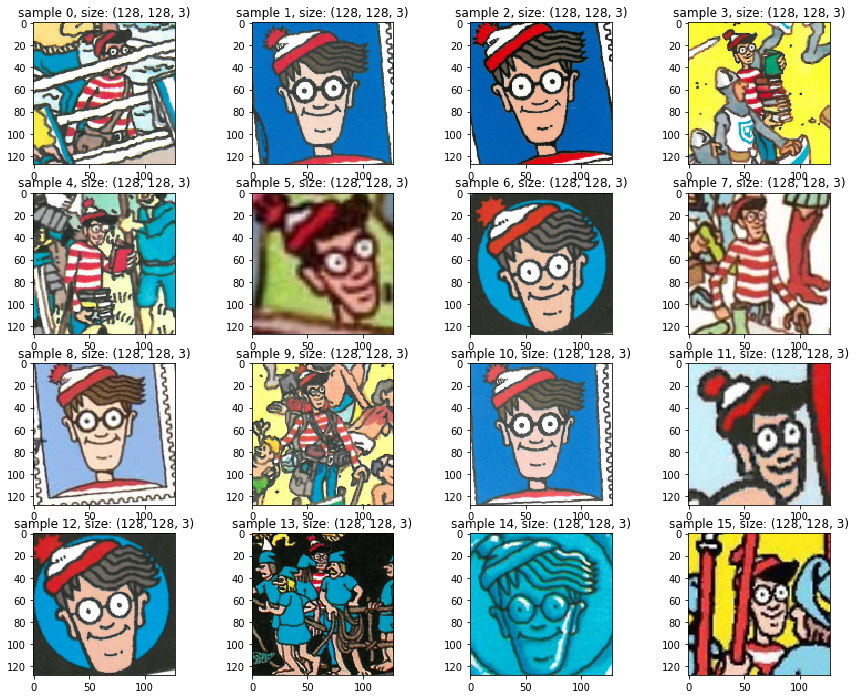
\includegraphics[width=0.4\linewidth]{figures/preprocess_waldo} 
    \hspace{1cm}
    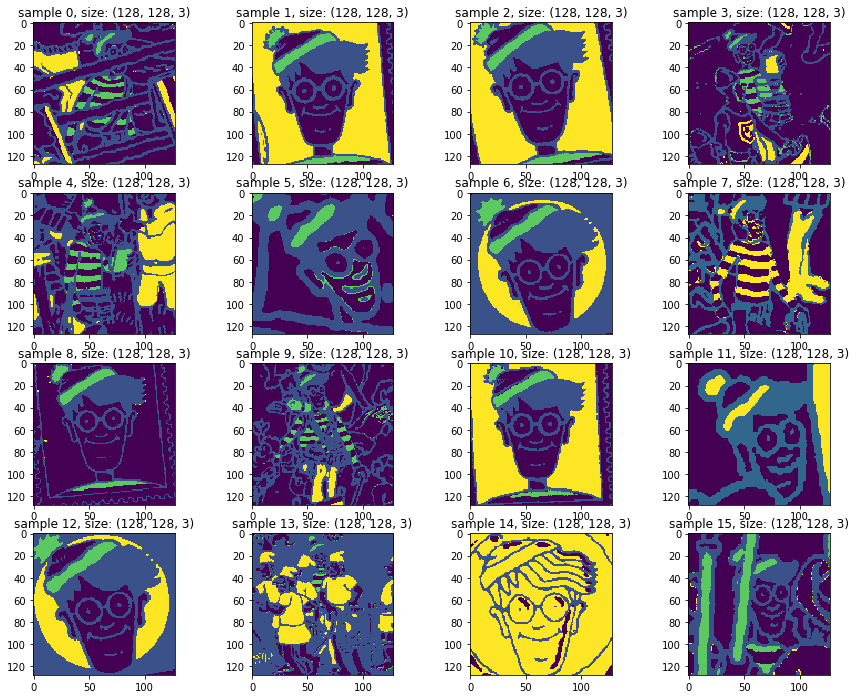
\includegraphics[width=0.4\linewidth]{figures/kmeans_waldo} 
    \caption{Preprocessed sample images for the waldo class. The left images are cropped and scaled to \( 128 \times 128 \) pixels.
    To the right the same images are shown after k-means preprocessing (originally gray-scaled, but color mapped for display purposes).}
    \label{fig:preprocessed-samples}
\end{figure}

To map the color images as robustly as possible to gray scale values we used a K-Means detector 
and assigned each of the modes an equally gray spaced color. 
K-Means works by intially choosing random starting points in the image and then projecting an area around them, calculating the "center of gravity"
of those inlier points and then shifting the new centroid to this "center of gravity". When repeating this
process until convergence, \( k \) such different means are found. This process results in a non-uniform quantization of the input image.
We use this property to train the K-Means classifier on a sample image of the \verb|wenda| class, which only 
shows the colors red, blue, black white. However we use \( k=5 \) to classify any color not lying in these four as a separate class, and then merge 
its results with the white color class. Then these four resulting classes colored centroids are mapped to uniformly
chosen values \( v \in [0, 255] \). This drastically reduces the complexity of the input images as can be seen in the right image in \autoref{fig:preprocessed-samples},
reducing input noise when processing the images with our feature descriptor in \autoref{subsec:implementation}.

Generating negative samples is done by randomly sampling regions of differing scales and positions from the provided training images.
In this process we additionally make sure that none of the proposed negative samples overlap with any of the ground truth annotations present in the images.
Then we scale these proposed negative samples to \( (128 \times 128 ) \) px and apply the filtering described in the above paragraph to each sample.
Since the negative samples are randomly generated, we can create arbitrary amounts of them. 
For our testing \( \approx15000 \) worked well. 
Additonal information in the exact size of the dataset is shown in \autoref{tab:dataset-stats}.


\begin{table}
    \centering
    \begin{tabular}{ccc}
        \toprule
        Class name & \#samples & percentage \\
        \midrule
        waldo & 137 &  1.01\% \\
        wenda & 43&  0.32\% \\
        wizard& 27&  0.20\% \\
        negative & 13315&  98.47\% \\
        \bottomrule
    \end{tabular}
    \caption{Dataset statistics for the SVM training}
    \label{tab:dataset-stats}
\end{table}


\subsection{Implementation}\label{subsec:implementation}

The pipeline for detecting the classes of a given bounding box are displayed in \autoref{fig:model-overview},
the first 3 steps of which are covered in \autoref{subsec:data-prep}. In the following paragraps we will focus on the
steps 4-7 of any detection and provide some details of interest in the implementation.

\begin{figure}[h]
    \centering
    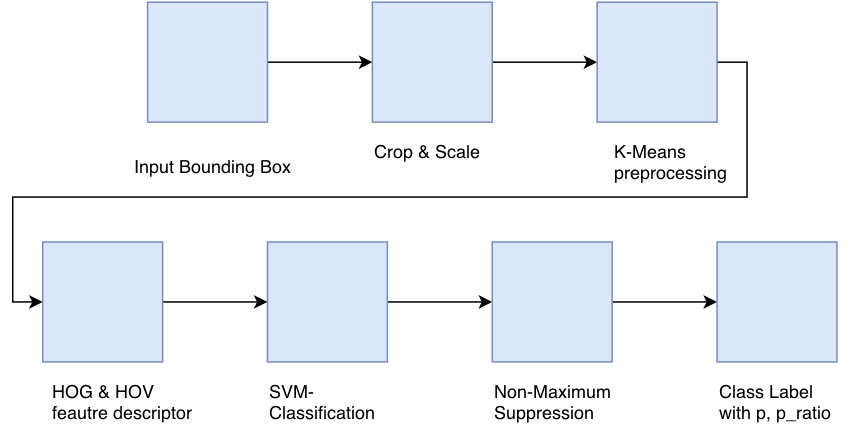
\includegraphics[width=0.9\linewidth]{figures/model_overview} 
    \caption{Schematic overview of the Waldo / Wenda / Wizard detection pileline}
    \label{fig:model-overview}
\end{figure}

\paragraph{HOG \& HOV feauture descriptor}
To capture shape and color information from the preprocessed sample images, we adopt a two-fold feature descriptor, 
which consists of the HOG descriptor and a histogramed version of the SIFT detector, we call HOV.

HOG works by first calculating the horizontal and vertical gradients in the image, which are then separated into
quadratic cells. From both a horizontal and vertical window, the magnitude and direction (radians or degrees) of the gradient get computed.
Then the magnitude is binned according to the corresponding direction. These bins then form a histogram for the cell.
This gives some invariance of the feature descriptor to slight pixel value changes. 
To also gives some spatial invariance, a set number of these histogramed cells are concatenated together. Which is repeated for each cell.
In a final step, the resulting feature vector is normalized with one of a multitude of possible norms. We decided to use the \( L_2 \)-Hys norm.

The HOV (Histograms over Values) descriptor works essentially the same (in fact most of the code is copied from the \verb|scikit-image| HOG implemenation),
with the only difference being that the initial histogram on each cell is not computed from the gradient of the input,
but rather the values of the input image inself.

Concatenating these two independently (with the same parameters) computed feature descriptors gives a good spatial and
value representation of the input images. The effect of which we evaluate in \autoref{subsec:results}.


\paragraph{SVM Classification}
Deciding which of the four classes \( \{waldo, wenda, wizard, negative \} \) should be assigned to any given window 
as confidently as possible, is handled by an ensemble of SVMs (Support Vector Machine)\cite{Hearst:1998:SVM:630302.630387}.

One SVM can only be used as a binary classifier, as explained in the remainder of this paragraph, but we require multiclass classification. 
Therefore we adopt a one-vs-one classification approach, where for each pair of classes \( \forall i,j: (c_i,c_j) \) a separate binary classifier is trained
and classifications are chosen by majority vote. We chose a one-vs-one approach versus a more traditional one-vs-rest approach as we a very unequal distribution of
positive an negative samples. Therefore any one-vs-rest classifier learns to only differentiate between the given class and negative samples. This showed itself 
during testing and classification performance could be improved by switching to a one-vs-one approach, even considering the additional computational expense.

Any one of the trained SVMs works by finding a hyperplane (plane in high dimensional feature space) which best separates the positive, from the negative samples.
The computation of this plane is performed iteratively by choosing a random starting plane and then finding dimensions which provide a good separation of the data. 
One such "good" separation is called a support vector of the hyperplane, giving the name Support Vector Machine. 
However this only works well if the data can be linearly separated by the dimensions of the input data. 
Since this is not always the case, and in general hard to analyse in high dimensional cases, we adopt an approach called RBF (Radial basis function) as proposed in\cite{10.1007/978-3-540-28647-9_85}.
Wang et. al. use this radial basis function to extend the data into another dimension, which in which it is hopefully linearly separable. Fitting this RBF kernel is also done at training time.
Traditionally SVMs can only give a distance of the sample from the decision hyperplane as a measure of confidence. 
However this metric is not always accurate and generally unbounded in value. Therefore we train another probabalistic model as proposed by Platt\ et.\ al.\cite{Platt99probabilisticoutputs}.
This applies cross validation on splits of the training data to calculate these probabilities, causing more computational expense during training.

Classification with the trained SVM is performed by first proposing a large amount of windows on the image and scaling each one to 
\( (128 \times 128) \) px, then performing the preprocessing steps outlined in \autoref{subsec:data-prep}. As the number of windows scales quadratically 
with image size, we process them in parallel across all cpus available. The windows in feature space then get given to the classifier, which predicts a label, probability \( p \) and the
\( p_{ratio} = p_{max} / p_{max - 1} \) value. Here \( p_{ratio} \) is used to give an indication of how confident the detector is in relation to all other classes with \( p_{max}, p_{max-1} \) being the two largest probabilities.
All predictions of the class \( negative \) get discarded, the other ones are passed to the Non-Maximum Suppression step.


\paragraph{Non-Maximum Suppression}
Since Classification is done for each window independently, and windows are densely sampled to provide good prediction accuracy, 
overlapping windows are possible. These get removed by performing Non-Maximum Suppression, which partitions all detections into groups according to their overlap.
Then for each of these groups, we chose the element with the maximum \( p \) value. Additional filtering is applied based on \( p_{ratio} > 1.5 \wedge p > 0.5 \) having to be true for each detection.
There values were determined experimentally to reduce the number of low confidence detections in the final result.

\paragraph{Class Label outputs}
In the final step, the detections after Non-Maximum Suppression are drawn to the input image and returned. 
This steps also includes potential drawing of ground truth boxes if provided

\subsection{Results}\label{subsec:results}

\begin{figure}[]
    \centering
    \begin{subfigure}{0.6\linewidth}
    \begin{tabular}{lcccc}
        \toprule
        class & precision & recall & \( F_1 \) score & \#samples \\
        \midrule
           waldo &  1.00 &  0.69 & \textbf{0.82} &  13 \\
           wenda &  0.80 &  0.57 & \textbf{0.67} &   7 \\
          wizard &  0.00 &  0.00 & \textbf{0.00} &   3 \\
        negative &  0.69 &  1.00 & \textbf{0.82} &  20 \\
        \bottomrule
    \end{tabular}
    \end{subfigure}
    \begin{subfigure}{0.35\linewidth}
    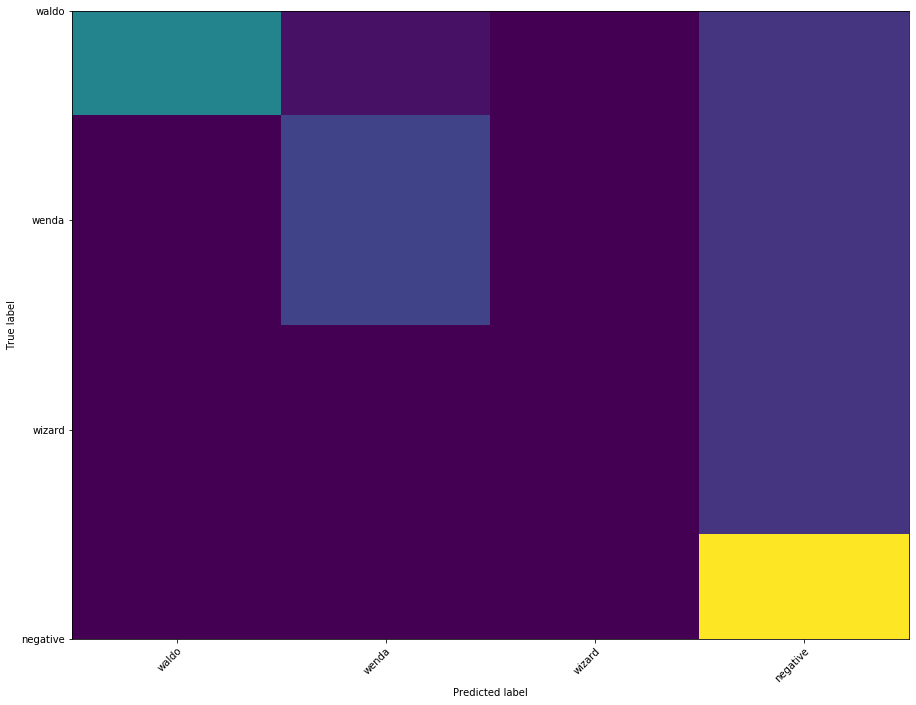
\includegraphics[width =\linewidth]{figures/confusion_matrix}
    \end{subfigure}

    \caption{Classification accuracies for waldo, wenda, wizard and negative classes on the HOG/HOV and SVM classifier
    with confusion matrix between the classes to the right.}
    \label{tab:classification_acc}
\end{figure}


% Present the results, both qualitatively (visualize) and quantitatively (specific numbers)..
% Analyze the results
Our Evaluation was is twofold, as we will firstly cover just the HOG/HOV \& SVM classifier itself, as evaluated on the 
validation set provided and then discuss how these results transfer over to the more general problem of detecting the classes in
full images.

For evaluation we use the now standard metrics in computer vision of precision, recall and their harmonic average the \( F_1 \) score.
They are defined as follows:

\begin{equation*}
    \text{precision} = \frac{|TP|}{|TP| + |FP|}  
    \quad
    \text{recall} = \frac{|TP|}{|TP| + |FN|}
    \quad
    F_1 = 2\cdot \frac{\text{precision} \cdot \text{precall}}{\text{precision} + \text{recall}}
\end{equation*}
Where \( TP \) is the set of \textbf{true positives}, intuitively detections of waldo, wenda, wizard or negative, which are also marked 
as the \textit{same} class in the validation set. 
\( FP \) is the set of \textbf{false positives}, intuitively cases where the detection is marked as the class under consideration, but actually belongs to any of the other ones.
\( FN \) is the set of \textbf{false negatives}, intuitively detections considered to be one of the classes other then the one under consideration, but which do belong to that class.

Considering the results achieved by the HOG/HOV \& SVM classifier on the validation set, 
we can see in \autoref{tab:classification_acc} that \( F_1 \) scores for the classes waldo and negatives are quite high, with
their precision and recall scores being opposites of each other. This suggests, that even although we trained a multiclass classifier, 
it is effectively classifying between the waldo and negative classes. This assumption also holds further when looking at the other
\( F_1 \) scores for wenda and wizard. They are acceptable for wenda, but none of the testing examples were classified as wizard, 
showing how our classifier is very unlikely to correctly detect wizard windows, which we will also discuss in the following paragraphs.

Gengeralizing our classifier to multiclass detector, we will now consider cropped images showing one ground truth class per image. 
Exemplary we have chosen three images to analyse from the dataset in \autoref{fig:detections}.
Already in the images one can see that overlap between the ground truth bounding boxes and the detections is not always large.
This is especially the case for \( I_1 \) containing wizard images, where the detected bounding box for wizard looks similar to the
ground truth box but is still a miss. We claim this could be classified as a close miss, hinting at a larger problem present in the dataset, 
of there being many possible windows which look very similar to true detections but are still considered negative even to the human eye. 
However the detections for \( I_2, I_3 \) are closer to the ground truth.

When comparing the performance of the HOG/HOV \& SVM approach to only using the HOG feature descriptor in \autoref{tab:class-iou}
one can verify the relevance of our extension to the HOG feature descriptor. As highlighted, the mean IoU (Intersection over Union) 
of ground truth bounding boxes to detection results is significantly improved when providing additional value information via the HOV descriptor, 
compared to only using the HOV descriptor.
However the greater IoU comes at the cost of additional computational expense, as highlighted by the mean computation time of each method.


\begin{figure}
    \centering
    \begin{subfigure}{0.3\linewidth}
    \stackunder[5pt]{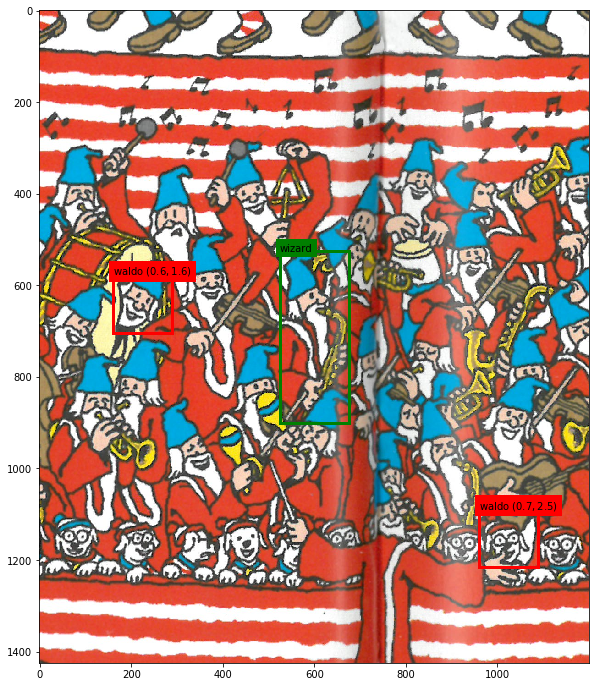
\includegraphics[height=4.5cm]{figures/crop_1}}{Wizard image: \( I_1 \)}
    \end{subfigure}
    \begin{subfigure}{0.3\linewidth}
    \stackunder[5pt]{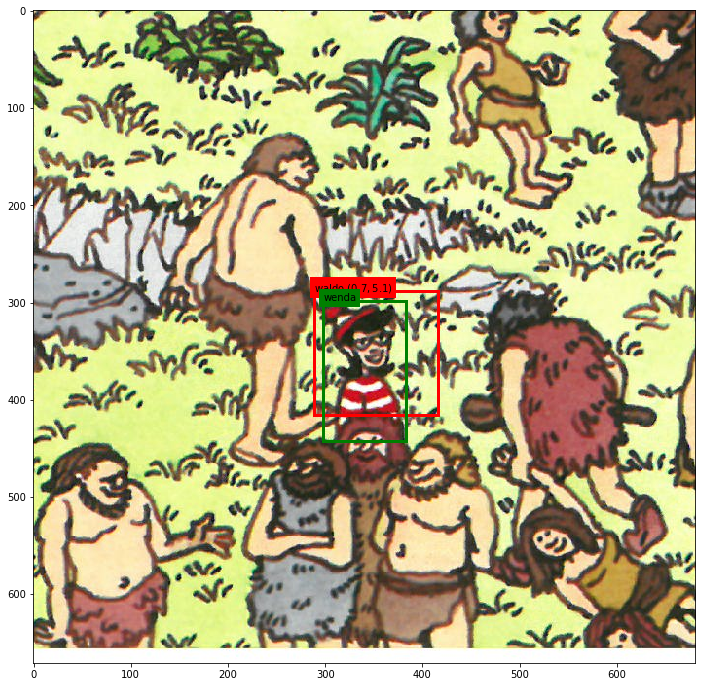
\includegraphics[height=4.5cm]{figures/crop_2}}{Wenda image: \( I_2 \)}
    \end{subfigure}
    \begin{subfigure}{0.3\linewidth}
    \stackunder[5pt]{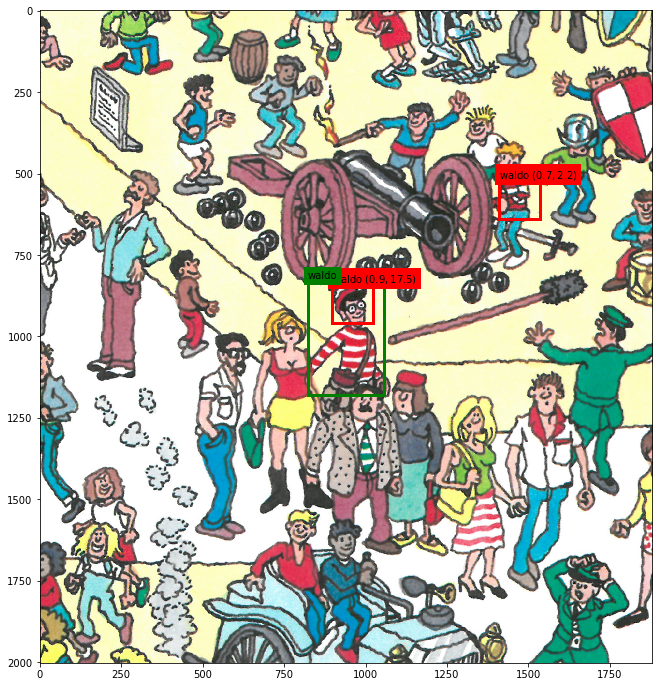
\includegraphics[height=4.5cm]{figures/crop_3}}{Waldo image: \( I_3 \)}
    \end{subfigure}
    \caption{Cropped wizard, wenda and waldo images \( I_1, I_2, I_3 \) with ground truth bounding boxes marked in green, 
    detections by HOG/HOV \& SVM in red with associated \( p, p_{ratio} \) values.}
    \label{fig:detections}
\end{figure}
\begin{table}
    \centering
    \begin{tabular}{lccccc}
        \toprule
        method & \( I_1 \) IoU & \( I_2 \) IoU & \( I_3 \) IoU & Mean IoU & Mean Time \\
        \midrule
        % Histogram correlation   & 0.8   & 0.8 & 0.8 & 1s \\
        HOG \& SVM              & 0.0   & 0.0 & 0.37 & \textbf{0.13} & 12.8 s \\
        HOG/HOV \& SVM          &  0.0  & 0.5 & 0.09 & \textbf{0.21} & 21.3 s \\
        \bottomrule
    \end{tabular}
    \caption{Comparison over cropped image regions (see \autoref{fig:detections}). Given is IoU with the ground truth bounding box for each image,
    as well as mean computation time.}
    \label{tab:class-iou}
\end{table}

\subsection{Discussion}
% Strengths and weakness in your method.

% Maybe we can talk about the methods we also tried but didn't work/didn't use for the final solution here(?)

% Strengths
% Schnell
% Accuracy für Waldo


Looking at the results our classifier produced for the test images, it appears that the internal
representation of our classes is not distinctive enough to achieve a very good classification performance.
An example for a classification error that underlines this hypothesis can be seen in \( I_1 \) of
\autoref{fig:detections}. The dog wears glasses and its colours match the typical appearance of
Waldo but other than that they don't have much in common. Nevertheless, it is classified as Waldo,
whereas the Wizard is not detected. Therefore we concluded that our classifier
might have picked up the most common features of Waldo like color and glasses but we did not use
enough training samples to learn enough other characteristics of Waldo so that he would stay
distinguishable from other characters in the illustrations whose appearance overlaps with his. The
same logic applies to Wenda as well. For Wizard on the other hand, we could not discover any
traits that made our algorithm detect non-Wizard characters because of a shared attribute. His
false positives appear very much random to us.

\section{Conclusion}
\begin{figure}
    \centering
    \begin{subfigure}{0.45\linewidth}
    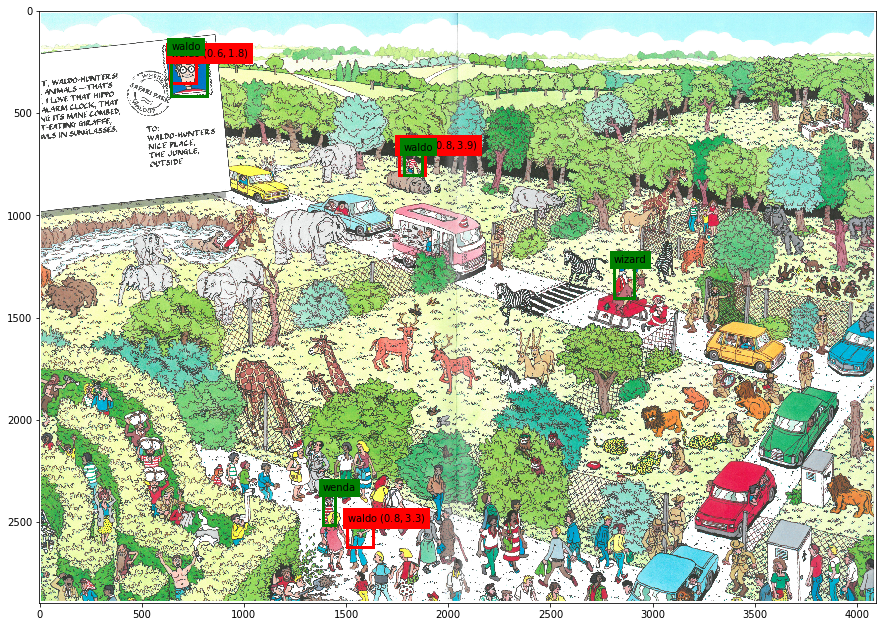
\includegraphics[width=\linewidth]{figures/detections_2}
    \end{subfigure}
    \begin{subfigure}{0.45\linewidth}
    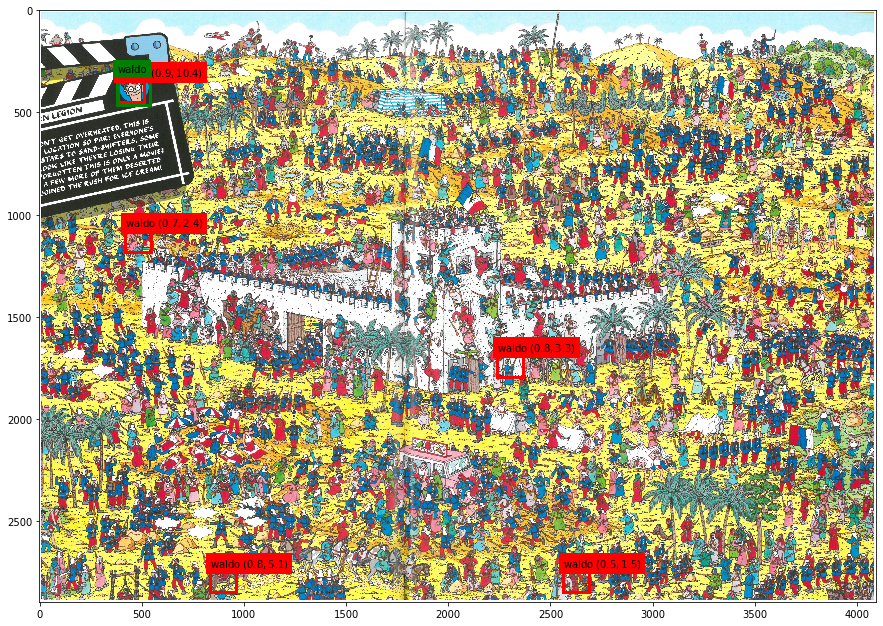
\includegraphics[width=\linewidth]{figures/detections_3}
    \end{subfigure}
    \caption{Detection on full size images of the validation set. Ground truth is shown in green, detections in red.}
    \label{fig:detections-img}
\end{figure}

In this project, we used several computer vision techniques and algorithms that we had
learnt in class, and put them into practice. Though our solution needs further work (see \autoref{fig:detections-img}) on the dismissal of
false positives, we manage to detect several instances of the characters of interest. By trying several
classification approaches simultaneously in the beginning of the project phase, we were able to reject those
which were less promising and could therefore concentrate our energy on improving the algorithm providing
the best results. The pursue of the idea to combine two feature descriptors lead to a significant increase
of the average performance of our classifier.

\pagebreak

\section{Group Information}

\begin{table*}[ht]
    \centering
    \begin{tabular}{lccc}
    \toprule
     Member & Student ID & Email & Contribution\\
    \midrule
    Maximilian Fruehauf& A0207441N & e0445541@u.nus.edu & HOG/HOV \& SVM, Report \\
    David Drews& Axx &e0454245@u.nus.edu & Haar Cascade, Report \\
    Choo Wen Xin& A0160465H & e0053347@u.nus.edu & Histogram Correlation, Report \\
    \bottomrule
    \end{tabular}
    \caption{Group member information.}
    \label{tab:dataset}
\end{table*}


\bibliographystyle{plain}

\bibliography{references}
 
\end{document}




